% !TeX root = ../main.tex

\chapter{系统详细设计与实现}

本章节基于系统概要设计部分,分别对模拟器四个主要功能模块的具体设计和实现细节进行阐述和说明。

\section{预加载模块的实现}

预加载模块主要实现了两个功能,指令集功能函数的翻译,以及解码器对指令列表的解析和注册。

对应单条汇编指令的取值,译码,执行过程,模拟器从PC地址读取一条32位的汇编指令,通过解码器进行解码,找到对应的功能函数,然后执行该功能函数。核心的数据结构就是指令类insn\_t,除了包含32位的uint数据成员来保存指令内容,还定义了一系列的接口,方便读取RISC-V指令格式所定义的指令码,寄存器,立即数等的位域信息。下面详细介绍模拟器对于指令类数据结构的定义和实现。
\begin{figure}[h]
    \centering
    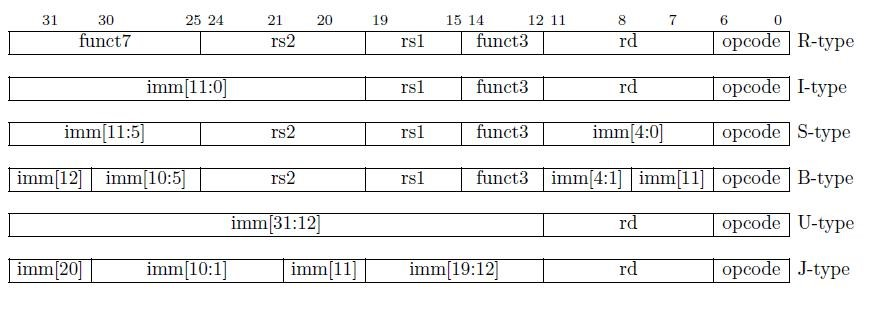
\includegraphics[width=1.0\textwidth]{insn-type.jpg}
    \caption{RISC-V32I 指令格式}
    \label{fig:insn-type}
\end{figure}


由前面的章节可以知道,RISC-V汇编指令的格式是非常明晰的,图~\ref{fig:insn-type}展示了RISC-V32I所包含的全部六种指令类型的格式。在实际编码过程中,编码位置的安排都是有意义的。例如3个寄存器索引号在不同指令格式中的编码位置是永远不变的,Rd在7-11bit位,Rs1在15-19bit位,Rs2在20-24bit位。即使有些指令中可能没有用到部分寄存器,比如第二个指令类型I-type中没有Rs2,但是Rs1和Rd的索引号也在对应的位置上。又例如在S-type里funct3在12-14bit位,与在R-type中的位置一致。操作码是所有指令格式都有的,而且位置不变,永远都是0-6bit位。得益于RISC-V指令类型的优秀设计理念,很容易抽象出指令类insn\_t,该类包含一个32位无符号数作为指令数据,另外定义统一的接口来获取RISC-V指令中的位域信息。结合读写寄存器的宏定义,可以方便地编写指令功能函数。该部分的实现较为简单,针对不同的位域信息,通过位运算获取相应的内容,主要为功能函数的实现提供接口。


区别于其他指令集架构的设计,RISC-V的译码过程是比对操作码和func位域信息,通过RISCV-OPCODES工具生成的头文件包含了所有标准指令集模块的指令格式信息,每条汇编指令都包含一对掩码(MASK)和匹配(MATCH)信息,译码过程是将指令内容与MASK取位与运算,得到的结果和MATCH一致表示是该条汇编指令。在模拟器实现过程中只需要为解码器开辟一块内存空间,存放(MATCH,MASK,insn\_t)的三元组即可,为了加快译码速度,在模拟器设计中,采用了哈希表的数据结构进行存储。综合上述接口定义,译码器取值,翻译,执行逻辑可以用伪代码表示为:
\begin{lstlisting}
    match = insn->GET_MATCH();           //获取指令MATCH,与掩码位与
    func = disassembler->GET_FUNC(match);//译码器指令翻译
    func(insn);                          //功能函数执行
\end{lstlisting}
预加载模块注册指令集,以及初始化解码器的流程如图~\ref{fig:decode-process}所示。
\begin{figure}[H]
  \centering
  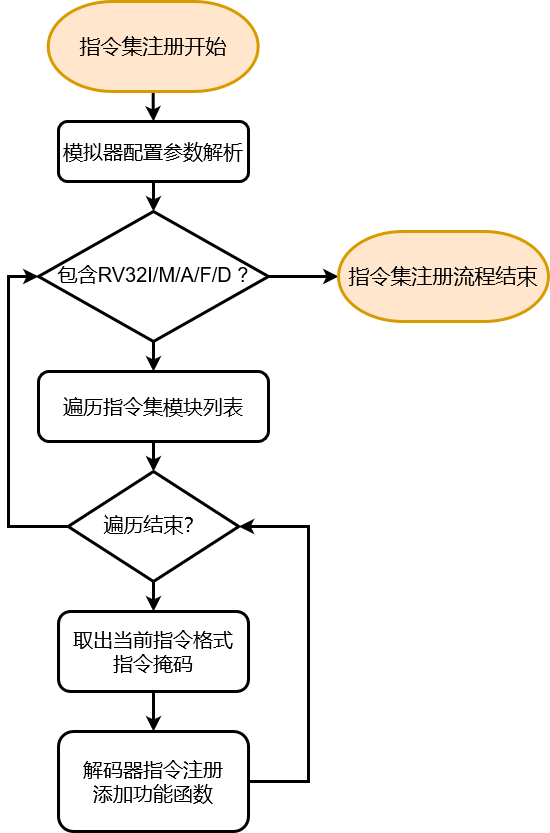
\includegraphics[width=0.5\textwidth]{decode-process.png}
  \caption{指令集模块注册流程图}
  \label{fig:decode-process}
\end{figure}


定义了指令数据结构和解码器之后,取指,译码的过程就完成了,接下来介绍执行步骤的核心内容,指令集功能函数的实现。


指令集功能函数是整个指令集模拟的核心部分,理论上说,汇编指令的功能函数需要和实际的硬件设计一一对应,由于硬件设计所参考的指令集架构版本已经定义了各个汇编指令的功能和具体行为,所以对于指令集的功能模拟只需要参照相应的指令集手册。本模拟器的设计过程依托于具体的芯片项目,由于大多数的硬件设计团队针对不同的性能指标往往会进行一些取舍,尤其是对于RISC-V这样的开源架构,实际的设计肯定会和官方版本有所出入,所以在模拟器的设计上还是需要参照硬件设计团队的代码。本次设计依托的芯片开发项目使用Chisel进行硬件设计,通过其生成的scala代码,可以指导模拟器指令功能函数的翻译。


\section{CPU和总线的实现}

上一节介绍了指令集模块的实现,从一个较高的抽象层次对模拟器的功能进行了定义,本节将详细介绍硬件的模拟细节,主要包含CPU内部的各个功能部件,以及CPU与片外通信的桥梁--总线的设计与实现。


\subsection{寄存器模拟}

寄存器是CPU内部用来存储数据的预定义单元,汇编指令的执行过程主要就是对寄存器和其他存储器的读写过程,因此对于寄存器的模拟需要做到精确且高效,为功能函数的编写提供良好的接口。


RISC-V体系结构中,定义了两类寄存器,整数和浮点寄存器XPR/FPR;控制与状态寄存器CSR(control and status register, CSR)。寄存器组的类图如图\ref{fig:csr_class}所示。
\begin{figure}[H]
    \centering
    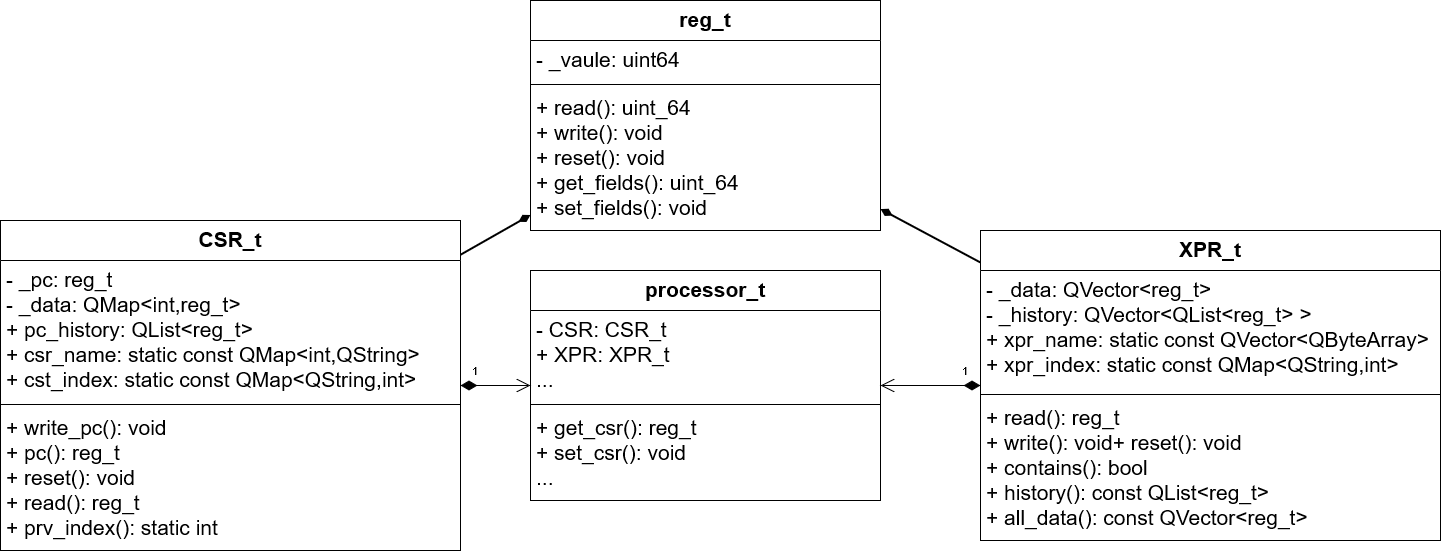
\includegraphics[width=1.0\textwidth]{csr_class.png}
    \caption{寄存器类图}
    \label{fig:csr_class}
\end{figure}


XPR/FPR均属于通用数据寄存器,在用户模式和机器模式下的访问方式一致,因此只需要将其定义为处理器类内部的公有成员,可以直接由处理器对象获取并修改。CSR寄存器主要由特权集指令进行位操作,表示CPU状态的改变,后续的调试模块也需要重点关注CSR的状态,因此在模拟实现上需要提供统一的接口,一方面为了简化指令集功能函数的实现,另一方面也可以节省参数传递等过程带来的性能损失。对于寄存器组的模拟,除了保存当前的运行时数据,还需要为后续的调试模块保存部分历史状态信息,比如程序计数器PC,状态寄存器MSTATUS等。总体设计上,寄存器组均封装在processor\_t类内部,其中通用寄存器组可以被处理器类对象直接调用,进行读写操作;CSR寄存器组被声明为类私有成员,对外提供get\_csr(),set\_csr()统一接口。将CSR寄存器访问权限,状态寄存器位域信息获取等操作封装在接口内部,这样就可以使指令集功能函数的实现不必关心具体的寄存器实现细节。根据RISC-V特权级架构文档,CSR寄存器接口的实现主要需要考虑三个因素:


1) 检查寄存器组所需的指令集模块支持。


2) 处理器当前权限模式检查。


3) CSR寄存器写入格式的检查。


以状态寄存器CSR\_MSTATUS为例。该寄存器格式如图~\ref{fig:mstatus}所示。状态寄存器持续跟踪和控制硬件线程的当前操作状态。在读写状态寄存器的过程中,需要检查VM,MPP,MPRV,PUM,MXR位是否有变化,如果上述的位域发生改变,表示处理器状态发生改变,需要在寄存器读写之前判断当前特权等级。
\begin{figure}[H]
    \centering
    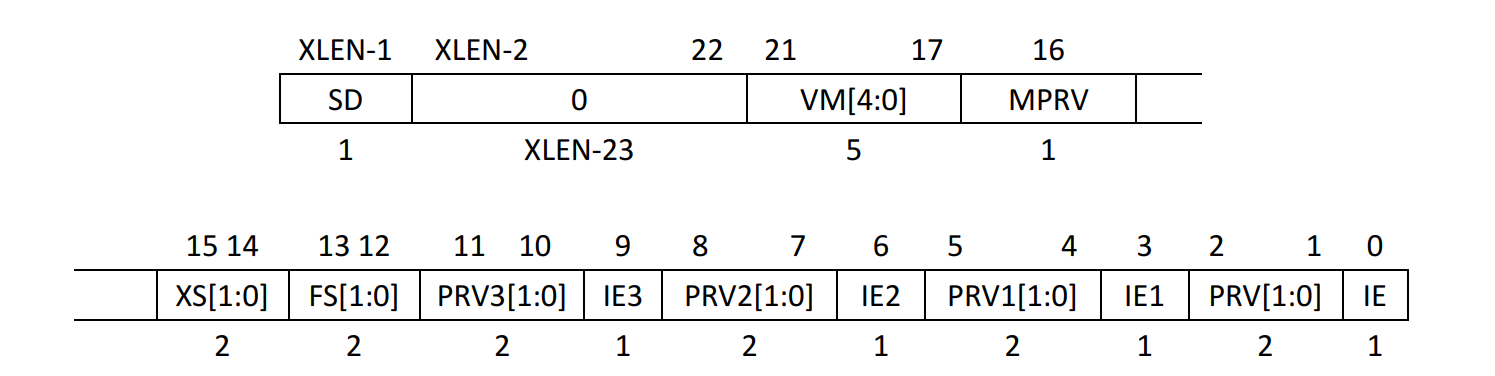
\includegraphics[width=1.0\textwidth]{mstatus.png}
    \caption{状态寄存器位域信息}
    \label{fig:mstatus}
\end{figure}


机器模式异常返回指令mret,用于从机器模式异常处理程序返回,是RISC-V架构中断流程的最后一条机器模式指令。该指令功能包含了上述的全部三种检查条件。下面以该指令为例,用伪代码详细说明寄存器模拟实现和指令功能函数的具体实现方式。mret的功能包括将PC还原为中断前的下一条指令(保存在mepc),将特权级设置成MPP位保存的值,将中断使能位MIE还原为MPIE位保存的值,最后将MPIE设置为1,完成从机器模式到用户模式的跳转。
\begin{lstlisting}
require_privilege(PRV_M);   //宏定义,用于检查当前状态寄存器特权模式
set_pc(p->get_state().mepc);//通过set\_pc()接口设置PC值
reg_t s = STATE.mstatus;    
reg_t prev_prv = get_field(s,MSTATUS_MPP);
s = set_field(s,MSTATUS_UIE<<prev_prv,get_field(s,MSTATUS_MPIE));
s = set_field(s,MSTATUS_MPIE,1); 
s = set_field(s,MSTATUS_MPP,PRV_U); //寄存器类set\_fields()接口置位
p->set_privilege(prev_prv);
p->set_csr(CSR_MSTATUS,s); //处理器类set\_csr()接口写CSR寄存器
\end{lstlisting}

在set\_csr()接口的实现中,需要对于CSR的读写进行检查,一方面是为了确保读写时所处的特权级模式是否支持读写,另一方面需要针对状态寄存器的改变做出相应的动作,比如tlb的清除等。
% \begin{lstlisting}
% case CSR_MSTATUS:
% {
%     if ((val ^ CSR.mstatus) & (MSTATUS_VM | MSTATUS_MPP | MSTATUS_MPRV | MSTATUS_PUM | MSTATUS_MXR))
%         mmu->flush_tlb();
%     reg_t mask = MSTATUS_SIE | MSTATUS_SPIE | MSTATUS_MIE | MSTATUS_MPIE
%                 | MSTATUS_SPP | MSTATUS_FS | MSTATUS_MPRV | MSTATUS_PUM
%                 | MSTATUS_MPP | MSTATUS_MXR ;
%     if (validate_vm(max_xlen, get_field(val, MSTATUS_VM)))
%     mask |= MSTATUS_VM;
%     CSR.mstatus = (CSR.mstatus & ~mask) | (val & mask);
%     bool dirty = (CSR.mstatus & MSTATUS_FS) == MSTATUS_FS;
%     dirty |= (CSR.mstatus & MSTATUS_XS) == MSTATUS_XS;
%     if (max_xlen == 32)
%         CSR.mstatus = set_field(CSR.mstatus, MSTATUS32_SD, dirty);
%     else
%         CSR.mstatus = set_field(CSR.mstatus, MSTATUS64_SD, dirty);
%     xlen = max_xlen;
%     break;
% }
% \end{lstlisting}

除了上述的寄存器,每个处理器对象都维护私有的PC程序计数器,初始化过程中PC被初始化为Bootrom地址。

\subsection{MMU和缓存模拟}

内存管理单元(Memory Management Unit, MMU)是一种负责处理CPU内存访问请求的计算机硬件。它的主要功能是进行虚拟地址到物理地址的转换(即虚拟内存管理)。
\begin{figure}[h]
    \centering
    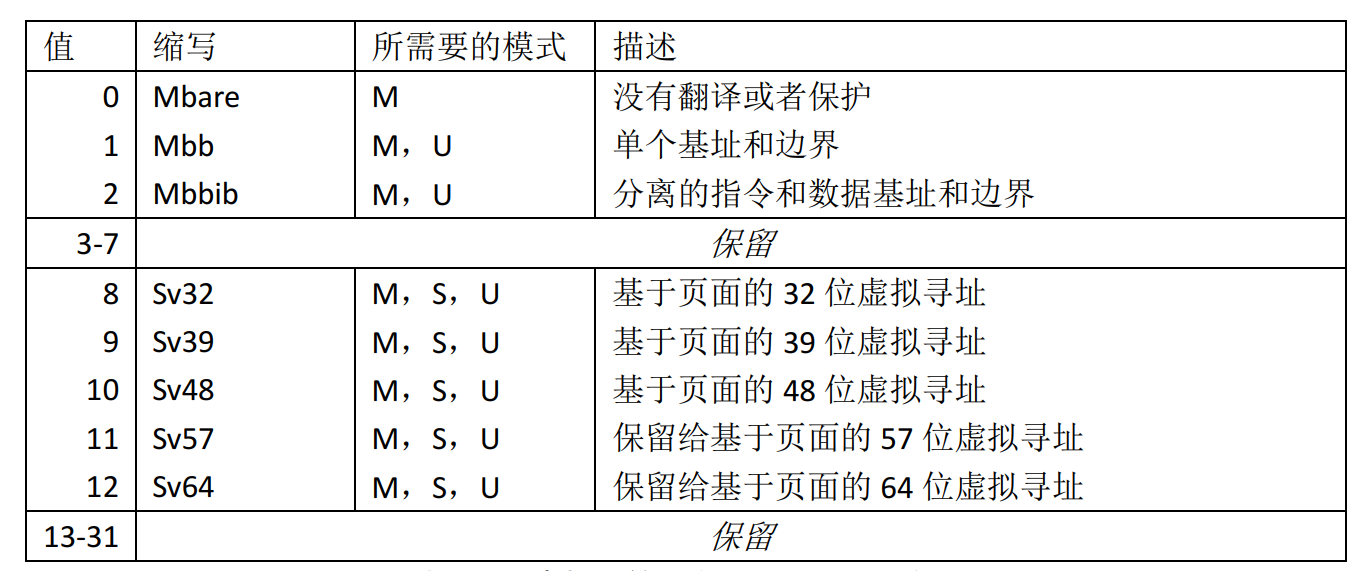
\includegraphics[width=0.9\textwidth]{VM.png}
    \caption{RISC-V虚拟化方案}
    \label{fig:VM}
\end{figure}

% 在MSTATUS状态寄存器中,虚拟化管理字段 VM[4:0]指示了当前活跃的虚拟化方案,包括虚拟存储器翻译和保护。图~\ref{fig:VM}给出了当前定义好的虚拟化方案。对于一个 RISC-V 硬件实现,只有 Mbare 模式是强制要求的,该模式没有存储器管理或翻译,因此所有的有效地址,无论其特权模式,都被认为是机器物理地址,是复位时进入的模式,理论上在该模式下不需要经过MMU进行地址翻译。Sv39 和 Sv48 是针对 RV64 系统的基于页面的虚拟存储器体系结构,提供了一个 39 位或 者 48 位的虚拟地址空间,被设计成支持现代管理员级操作性,包括基于 Unix 的系统。Sv39、 Sv48 需要实现支持 M、 S 和 U 特权级。
在RISC-V体系结构中,与MMU有关的CSR寄存器主要有控制与状态寄存器MSTATUS和页表基址寄存器SPTBR。MSTATUS的VM位域记录了当前的虚拟化方案,图~\ref{fig:VM}给出了RISC-V架构定义的所有虚拟化方案。对于一个 RISC-V 硬件实现,只有 Mbare 模式是强制要求的,该模式下地址是直接映射,理论上不需要经过MMU进行地址翻译,Sv39和Sv48分别表示39位和48位的虚拟地址空间,本模拟器支持上述三种虚拟化方案,但是为了实现方便,所有的主存访问请求都需要经过MMU,通过MMU模块的统一接口进行访存,当mstatus寄存器VM位为0时,无需进行地址翻译。以Linux内核加载过程中从物理地址向虚拟地址过渡的逻辑可以看出,当内核支持MMU时,会进入到relocate代码段进行页表基地址寄存器的初始化,内核通过setup\_vm()函数进行了首级页表的加载,然后在relocate段计算了首级页表基地址,写入sptbr寄存器,然后通过一条mret指令跳出机器模式,以后首级页表会常驻内存,接下来就全是加载虚拟地址了,MMU开始工作。以下列出了Linux V5.10版本的relocate代码段,由于Linux内核对于RISC-V架构的支持依据的是RISC-V官方给出的最新指令集版本,所以对于芯片设计厂商的具体硬件通常不能够直接适配,经常需要对软件进行微调,以适应硬件架构设计。
\begin{lstlisting}{}
    #ifdef CONFIG_MMU
    relocate:
        li a1, PAGE_OFFSET
        la a2, _start
        sub a1, a1, a2
        add ra, ra, a1
        la a2, 1f
        add a2, a2, a1
        csrw CSR_TVEC, a2
        srl a2, a0, PAGE_SHIFT
        li a1, SATP_MODE
        or a2, a2, a1
        la a0, trampoline_pg_dir
        srl a0, a0, PAGE_SHIFT
        or a0, a0, a1
        sfence.vma
        csrw sptbr, a0
    .align 2
    1:
        /* Set trap vector to spin forever to help debug */
        la a0, .Lsecondary_park
        csrw CSR_TVEC, a0
        /* Reload the global pointer */
    .option push
    .option norelax
        la gp, __global_pointer$
    .option pop
        csrw sptbr, a2
        sfence.vma
        ret
    #endif /* CONFIG_MMU */    
\end{lstlisting}


在本模拟器的实现中,MMU模块包含了快表TLB,加速地址翻译,本质上就是开辟了一片内存用来存放翻译过的地址内容,为了方便起见,只实现了直接映射的TLB。另外,将iCache,dCache的功能也一并放到MMU模块中,不再实现单独的缓存硬件模块,缓存采用直写的方式。这样的设计和真实硬件的差异很大,会导致缓存模拟的不准确。考虑到本模拟器并不进行缓存相关的性能模拟,所以可以忽略这部分的差别,在功能模拟上没有影响。MMU模块对取值做特殊处理,取值首先会查找iCache,当iCache未命中时,退化为其余类型的访存。访存请求通过模板函数提供的统一的接口load/store进行请求,通过模板可以忽略具体的数据类型,在功能函数的实现中也可以更加方便的使用,直接调用MMU的接口对存储单元进行操作。
% 模板函数定义如下:
% \begin{lstlisting}{}
%     template<class T>
%     inline T load(reg_t addr)
%     {
%         if (addr & (sizeof(T)-1))
%             throw trap_t(trap_load_address_misaligned,addr);
%         reg_t vpn = addr >> PGSHIFT;
%         if (likely(tlb_load_tag[vpn % TLB_ENTRIES] == vpn))
%             return *(T*)(tlb_data[vpn % TLB_ENTRIES] + addr);
%         T res;
%         load_slow_path(addr, sizeof(T), (uint8_t*)&res);
%         return res;
%     }    
% \end{lstlisting}


MMU接收到访存请求后,首先会检查地址对齐,然后通过页大小计算出虚拟页号,TLB的具体实现是一个哈希表,采用直接映射,如果TLB未命中,则进入load\_slow\_path()逻辑,需要查找页表,这部分的地址翻译过程封装在MMU类中,在翻译之前首先确认地址范围是否是MMIO地址范围,如果是,就将访存任务转移给总线处理,后续将详细说明MMIO的流程。综上,整个MMU和缓存模块的功能实现都封装到MMU类内部,访存请求的活动图如图~\ref{fig:slow_path}所示。
\begin{figure}[H]
    \centering
    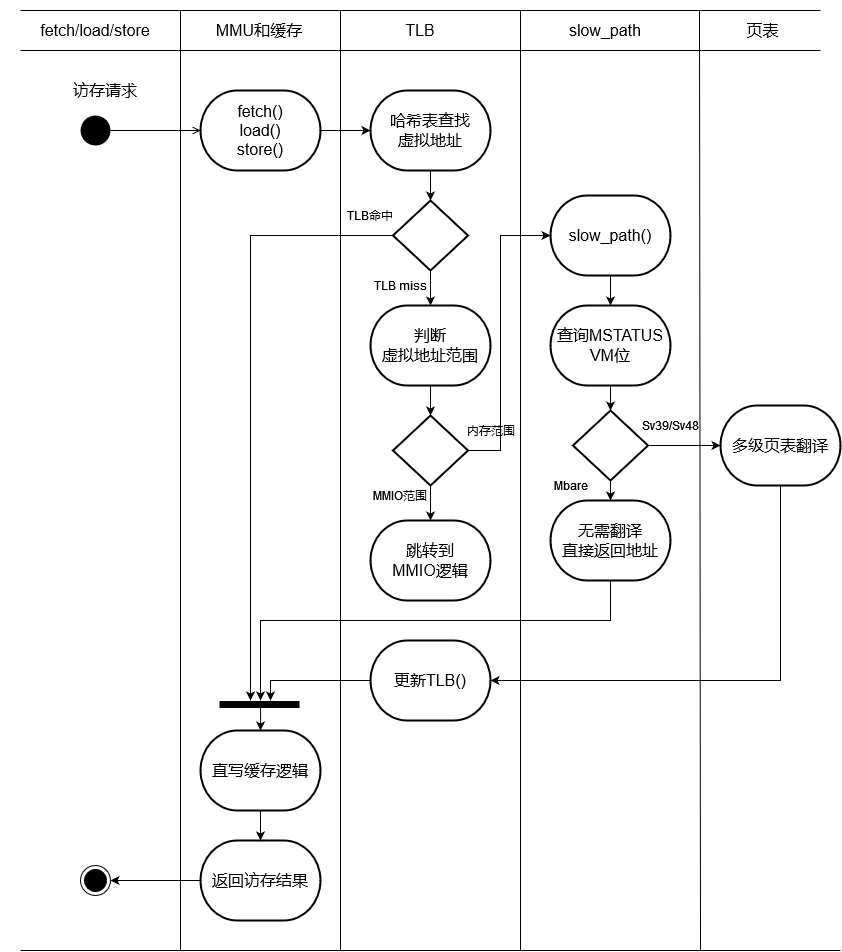
\includegraphics[width=0.95\textwidth]{slow_path.png}
    \caption{访存请求活动图}
    \label{fig:slow_path}
\end{figure}

\subsection{总线和I/O模拟}
总线是CPU与外部设备进行数据交换的桥梁,按照功能有不同的总线类型划分,本模拟器对总线设备进行了功能抽象,将总线设计为某一块物理地址区间内的IO控制器,提供统一接口,处理CPU和内存映射的IO设备之间的通信。


总线在模拟器初始化的过程中会根据配置挂载设备,在总线类bus\_t中维护一个物理地址和设备类对象的map,模拟器在接收到访存请求时,首先检查物理地址是否是主存地址范围,不在主存地址区间内的I/O请求都是内存映射的I/O请求(Memory-Mapped I/O, MMIO),模拟器将调用总线设备的IO接口,对内存映射的外设进行读写操作。

模拟器根据物理地址划分为主存,和内存映射的IO设备,图~\ref{fig:mmap}是SiFive公司提供的内存映射参考。本模拟器的总线设备需要处理的内存映射空间就是0x00000000-0x80000000,提供这块内存区间上的IO模拟。总线设备可以挂载多种通过内存映射的IO设备,某些具有特殊用途的寄存器也能够挂载在总线,比如timecmp寄存器,ipi寄存器。
\begin{figure}[H]
    \centering
    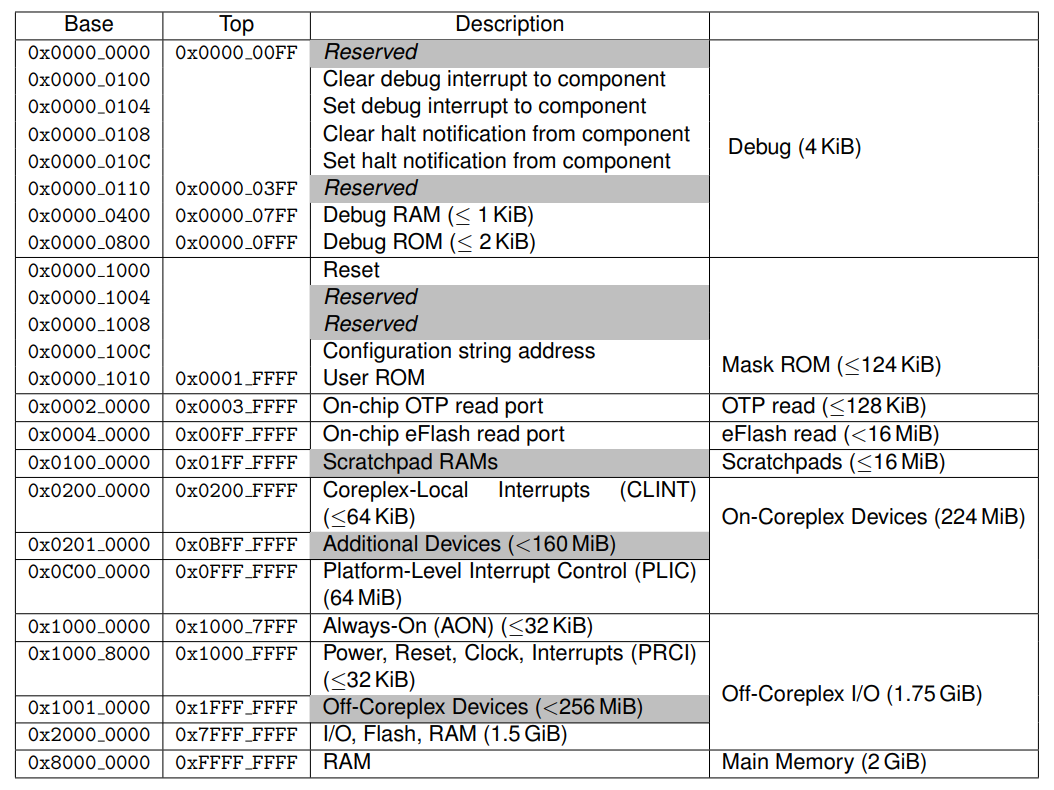
\includegraphics[width=0.8\textwidth]{mmap.png}
    \caption{SiFive公司的内存映射方案}
    \label{fig:mmap}
\end{figure}


总线设备的类图如图\ref{fig:bus_class}所示。所有设备都继承自抽象基类abstract\_device\_t,在总线类bus\_t中维护一个设备数组,统一管理挂载到总线的MMIO设备,比如图中的RTC设备,此类设备的IO均需要通过总线对象的MMIO接口与处理器进行通信。
\begin{figure}[H]
    \centering
    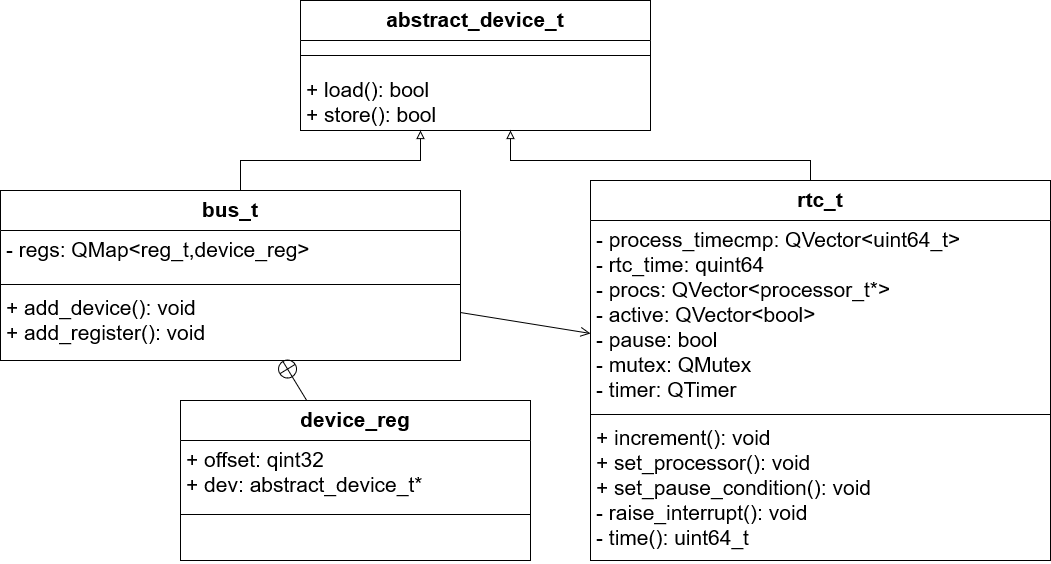
\includegraphics[width=0.8\textwidth]{bus_class.png}
    \caption{总线设备类图}
    \label{fig:bus_class}
\end{figure}


所有支持安全启动的CPU都会有一个Bootrom固件。CPU在通电之后执行的第一条指令就在Bootrom的入口,因此Bootrom拥有最高的执行权限,也就是机器模式M-mode。它将初始化Secure Boot安全机制,加载Secure Boot Key等密钥、从存储器加载并验证第一阶段加载程序(First Stage Bootloader, FSBL),最后跳转进FSBL中。本次芯片设计项目也包含了该部分的设计,但是由于安全启动过程涉及到部分保密信息,本文将不涉及FSBL的加载和验证过程,Bootrom固件程序仅仅用来跳转置目标程序入口。具体的实现方式包括以下的步骤,首先在配置中读取Bootrom的地址,默认0x1000,然后初始化Bootrom设备,填写Bootrom固件内容,总线对象使用add\_device()接口将物理地址0x1000和Bootrom设备对象的映射保存在字典中。本模拟器的Bootrom程序内容如图所示,包含两条汇编指令:
\begin{lstlisting}{}
    auipc	t0, 0x7ffff
    jr 	t0
\end{lstlisting}
模拟器启动后,PC初始化位Bootrom固件地址,即0x1000,MMU检测到该地址在MMIO区间内,将访存请求转移给总线,总线对象使用MMIO接口找到对应的设备对象Bootrom,读取到Bootrom的两条指令,处理器在机器模式执行上述两条指令,跳转到主存起始位置0x80000000,即目标程序的入口地址。接下来的一系列指令执行由目标程序决定,主要包括Bootloader的reset vector以及加载Linux内核的过程。

mmio的通信流程如图~\ref{fig:mmio}所示。
\begin{figure}[H]
    \centering
    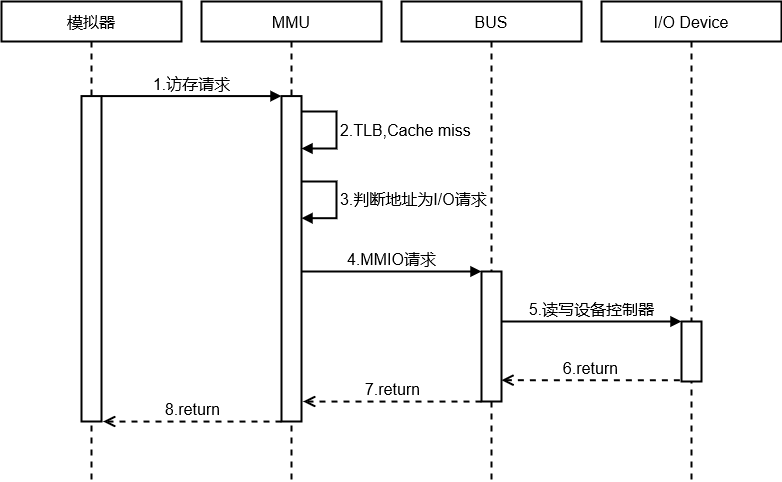
\includegraphics[width=0.8\textwidth]{mmio.png}
    \caption{MMIO请求流程}
    \label{fig:mmio}
\end{figure}


\section{中断系统的实现}

在CPU运行过程中,存在两种指令流程,一种是常规的逻辑控制流,包括顺序的指令流和分支跳转;另一种称为异常控制流,用来响应处理器状态的某些变化,表现为中断或异常。之前的章节已将介绍了CPU指令控制流程的模拟,其中包括了响应中断的逻辑,CPU在取值之前检查当前是否有中断信号,根据状态寄存器判断是否响应中断,进入异常控制流逻辑。本节将详细阐述模拟器中断系统的实现。包括平台级中断控制器PLIC以及部分中断源的模拟。


RISC-V一共有两大类的中断类型:局部中断(Local Interrupts)以及全局中断(Global Inerrupts)。局部中断是指直接与硬件线程相连的中断,可以直接通过CSRs当中的xcause(mcause、scause、ucause)中的值获取中断的类型。在局部中断当中,只有两种标准的中断类型:计时中断(timer)以及软件中断(software)。全局中断实际上就是外部中断(External Interrupts)。它与平台级中断控制器PLIC相连。实际上全局中断在多个硬件线程的情况下最为常用,PLIC用于对外部中断进行仲裁,然后再将仲裁的结果送入核内的中断控制器。
RISC-V 架构中规定了一些硬件行为来实现异常事件的响应和处理,这些行为通过控制状态寄存器来反应异常事件信息。涉及到如下几个寄存器,见表~\ref{tab:csr}。
\begin{table}[h]
  \centering
  \caption{中断相关的寄存器}
  \label{tab:csr}
  \begin{tabular}{cl}
    \toprule
寄存器	& \multicolumn{1}{c}{功能}\\
    \midrule
    mstatus	& \multicolumn{1}{m{9cm}}{状态寄存器,保存全局中断使能等信息。}\\ \hline
    mie	& \multicolumn{1}{m{9cm}}{外部中断使能寄存器}\\ \hline
    mtvec	& \multicolumn{1}{m{9cm}}{异常入口基地址寄存器}\\ \hline
    mscratch & \multicolumn{1}{m{9cm}}{上下文切换时用于保存当前的指针信息}\\ \hline
    mepc & \multicolumn{1}{m{9cm}}{异常 PC 寄存器,现场保护时保存PC值}\\ \hline
    mcause & \multicolumn{1}{m{9cm}}{异常原因寄存器}\\ \hline
    mip	& \multicolumn{1}{m{9cm}}{中断悬挂寄存器,标识中断信号pending}\\ \hline
    mbadaddr & \multicolumn{1}{m{9cm}}{异常原因辅助信息寄存器}\\
    \bottomrule
  \end{tabular}
\end{table}

本模拟器实现了这部分的硬件行为,包括中断源的产生,和中断响应,下面进行详细的介绍。在处理器类内定义了两个uint64型数据,分别用来表示时钟中断和外部中断的pending,总线上挂载的设备可以直接对这两个pending数据进行设置,用来模拟外设”异步”的中断请求发起。处理器在下一个取值周期之前,使用try-catch语句来处理可能的中断响应,如果处理器决定响应中断,就会抛出一个trap\_t类型的异常,进入到响应中断的异步逻辑。trap\_t的定义如下:
\clearpage
\begin{lstlisting}{}
    class trap_t
    {
    public:
        trap_t(){}
        trap_t(reg_t type):cause(type),addr_valid(false){}
        trap_t(reg_t type,quint64 addr):cause(type),addr_valid(true),addr(addr){}
        reg_t cause;
        bool addr_valid;
        quint64 addr;
        static QMap<reg_t,QString> names;
        static quint64 delegable_exceptions;
        QString &name(){return names[cause];}
    };        
\end{lstlisting}

抛出异常后,处理器将根据状态寄存器以及异常信息决定是否响应中断,CPU异常处理的流程如图~\ref{fig:interrupt}所示。
\begin{figure}[H]
    \centering
    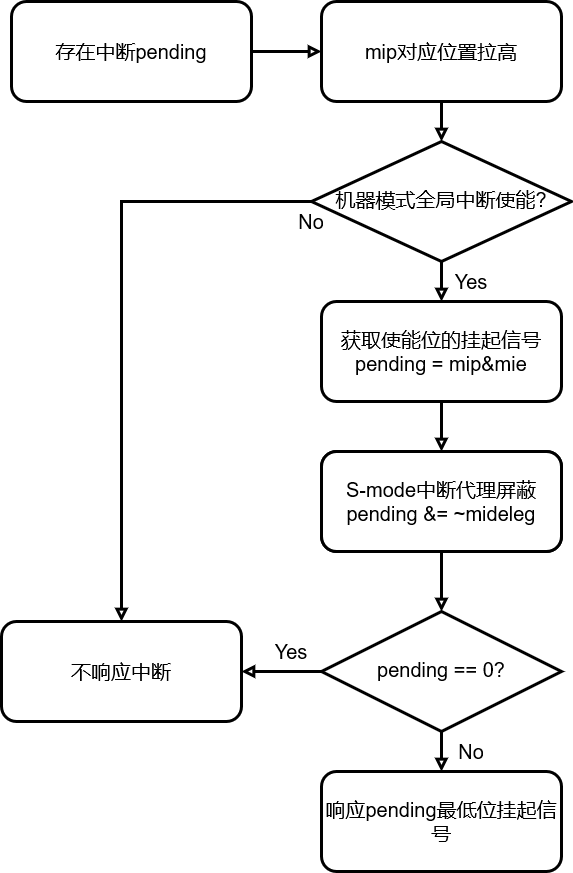
\includegraphics[width=0.5\textwidth]{interrupt.png}
    \caption{处理器响应中断流程}
    \label{fig:interrupt}
\end{figure}

模拟器抛出异常后,根据捕获到的trap\_t,进入中断处理流程。RISC-V特权架构对这部分的处理器行为做了一定规范,本模拟器的实现也参照了特权架构定义。


1) 根据处理的中断类型将信号源编号记录到mcause寄存器中;


2) 地址不对齐或者发生访问异常,将导致错误的指令部分保存到mbadaddr;


3) 更新状态寄存器mstatus,记录中断处理前的状态;


4) 保存当前PC到 mepc寄存器中,以便于处理完中断后返回;


5) 停止当前执行程序流,设置PC为mtvec中断向量表入口地址并开始执行。


以上就是中断产生和响应过程对应的处理器硬件行为模拟,接下来将着重阐述平台级中断控制器PLIC的实现。


\subsection{PLIC模拟}

PLIC的功能是接受外部中断源发出的中断信号,对中断请求进行裁决,将裁决结果和外部中断信号发送给处理器。本模拟器参照了SiFive公司的PLIC规范文档进行设计,通过设备树挂载PLIC设备,通过对内存映射的寄存器进行读写来配置PLIC。根据上一章的PLIC概要设计,将中断源和中断目标分别抽象成plic\_dev\_info\_t类和plic\_core\_info\_t类,整体的PLIC中断控制器的设备类图如图~\ref{fig:plic-class}所示。
\begin{figure}[H]
    \centering
    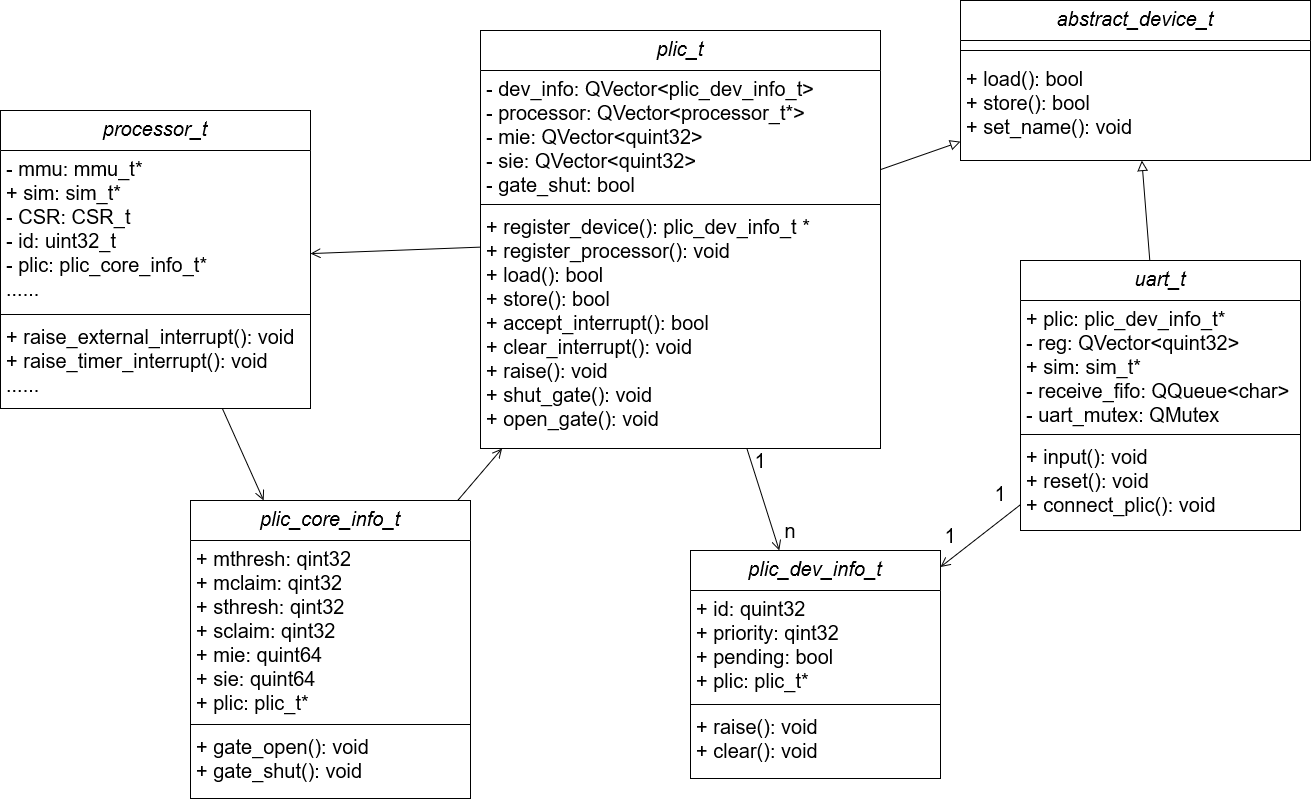
\includegraphics[width=1.0\textwidth]{plic-class.png}
    \caption{PLIC设备类图}
    \label{fig:plic-class}
\end{figure}
以串口控制器类uart\_t为例,在外设的模拟实现中,通过connect\_plic()接口初始化设备类中的plic\_dev\_info\_t对象,并将自身挂载到PLIC设备上,后续设备的IO请求可以通过plic\_dev\_info\_t::raise()接口发送到PLIC设备,模拟了闸口的功能。PLIC设备类型plic\_t中定义了accept\_interrupt()接口用来拉高对应设备的IP寄存器,plic\_t::raise()接口实现了中断信号裁决,将裁决后的中断ID写入mclaim和sclaim寄存器,并且向处理器发送外部中断信号,当处理器响应中断时,会读取这两个寄存器的值,然后进入中断向量表,查找对应的中断处理函数,通常会调用定义在内核drives目录下的驱动程序。中断处理结束后,处理器会给PLIC core发送中断完成信息,具体的动作就是对PLIC中断源指定位置claim寄存器发送一条store指令,根据SiFive公司给出的规范,中断源ID为n的的claim/complete寄存器内存映射位置等于(PLIC基地址+0x200004+0x1000*n),因此该位置进行store请求时直接调用处理器对应plic\_core\_info\_t对象的gate\_open()接口来打开闸口。此时PLIC完成一次外部中断请求周期,可以发起下一次的中断请求。




\subsection{RTC模拟}

RISC-V架构还定义了硬件线程内的局部中断,局部中断控制器(Core-Local Interruptor, CLINT)是一个存储器地址映射模块,CLINT只负责处理软件中断和时钟中断,因为这两个中断是RISC-V架构中定义的,经过CLINT不需要进行任何的仲裁,直接将中断信号写入对应的寄存器内即可。软件中断只需要向CLINT的MSIP0或者SSIP0寄存器的最高位写1即可,处理完中断后,将其置为0,这样就能够清除掉软件中断的标志位。计时器中断作为RISC-V内核特有的中断,其用法就是往MTIMECMP或者STIMECMP中写特定的值,当mtime达到该值时产生中断,此时继续填写特定的tick就可以继续产生下个中断,反复如此,便可产生周期性的时钟中断。想要模拟时钟中断,需要宿主机产生时钟源,这部分的实现使用了Qt类库中的QTimer类对象,周期性地调用RTC类的increment()接口来模拟时钟的发生,当到达时钟中断条件是,通过MMIO接口更新RTC设备的TIMECMP寄存器,并调用raise\_interrupt()接口抛出异常,拉高时钟中断pending位,模拟时钟中断的发生。在下一指令周期,处理器接收时钟中断信号,进入中断处理流程。

% \subsection{外部中断源模拟}


\section{调试模块和UI实现}
调试模块能够提供断点设置,单步执行,寄存器/内存查询等功能。UI显示界面主要包含了断点设置窗口,查询窗口和执行交互窗口。本模块使用Qt的UI Designer工具进行开发,通过拖拽摆放各种窗口控件并进行属性设置,观察界面整体效果,可以方便地进行可视化界面的设计。另外QtWidget库还提供了信号(Signals)和槽(Slots)机制,用于对象间通信,只需要在对应窗口子类化widgets来添加自定义信号,然后实现自定义的槽函数,连接到该信号即可。在本模拟器的实现中,主要的对象间通信就是前端窗口对象和后端模拟器对象间的通信,因此只需要定义一组双向的信号和槽就能够满足通信需求。


前端UI窗口和后端模拟器之间的信号定义如下:
\begin{lstlisting}{}
    enum sim_cmd
    {
        sim_cmd_pause_sim,
        sim_cmd_run_sim,
        sim_cmd_run_sim_silently,
        sim_cmd_step_sim,
        sim_cmd_reset_sim,
        sim_cmd_access_memory,
        sim_cmd_set_breaks,
        sim_cmd_key_input,
        sim_cmd_mailbox_input
    };
        
    enum window_cmd
    {
        window_cmd_update_reg,
        window_cmd_update_mem,
        window_cmd_sim_output,
        window_cmd_gst_output,
        window_cmd_pause_sim,
        window_cmd_update_mailbox
    };          
\end{lstlisting}
其中sim\_cmd\_key\_input和sim\_cmd\_mailbox\_input信号分别用来模拟UART和mailbox外部中断源信号。其余信号用于断点和查询信息的交互,以及模拟器单步运行等流程的控制。
        
        
通过UI Designer设计的模拟器前端整体界面如图~\ref{fig:zhenti}所示。
\begin{figure}[h]
    \centering
    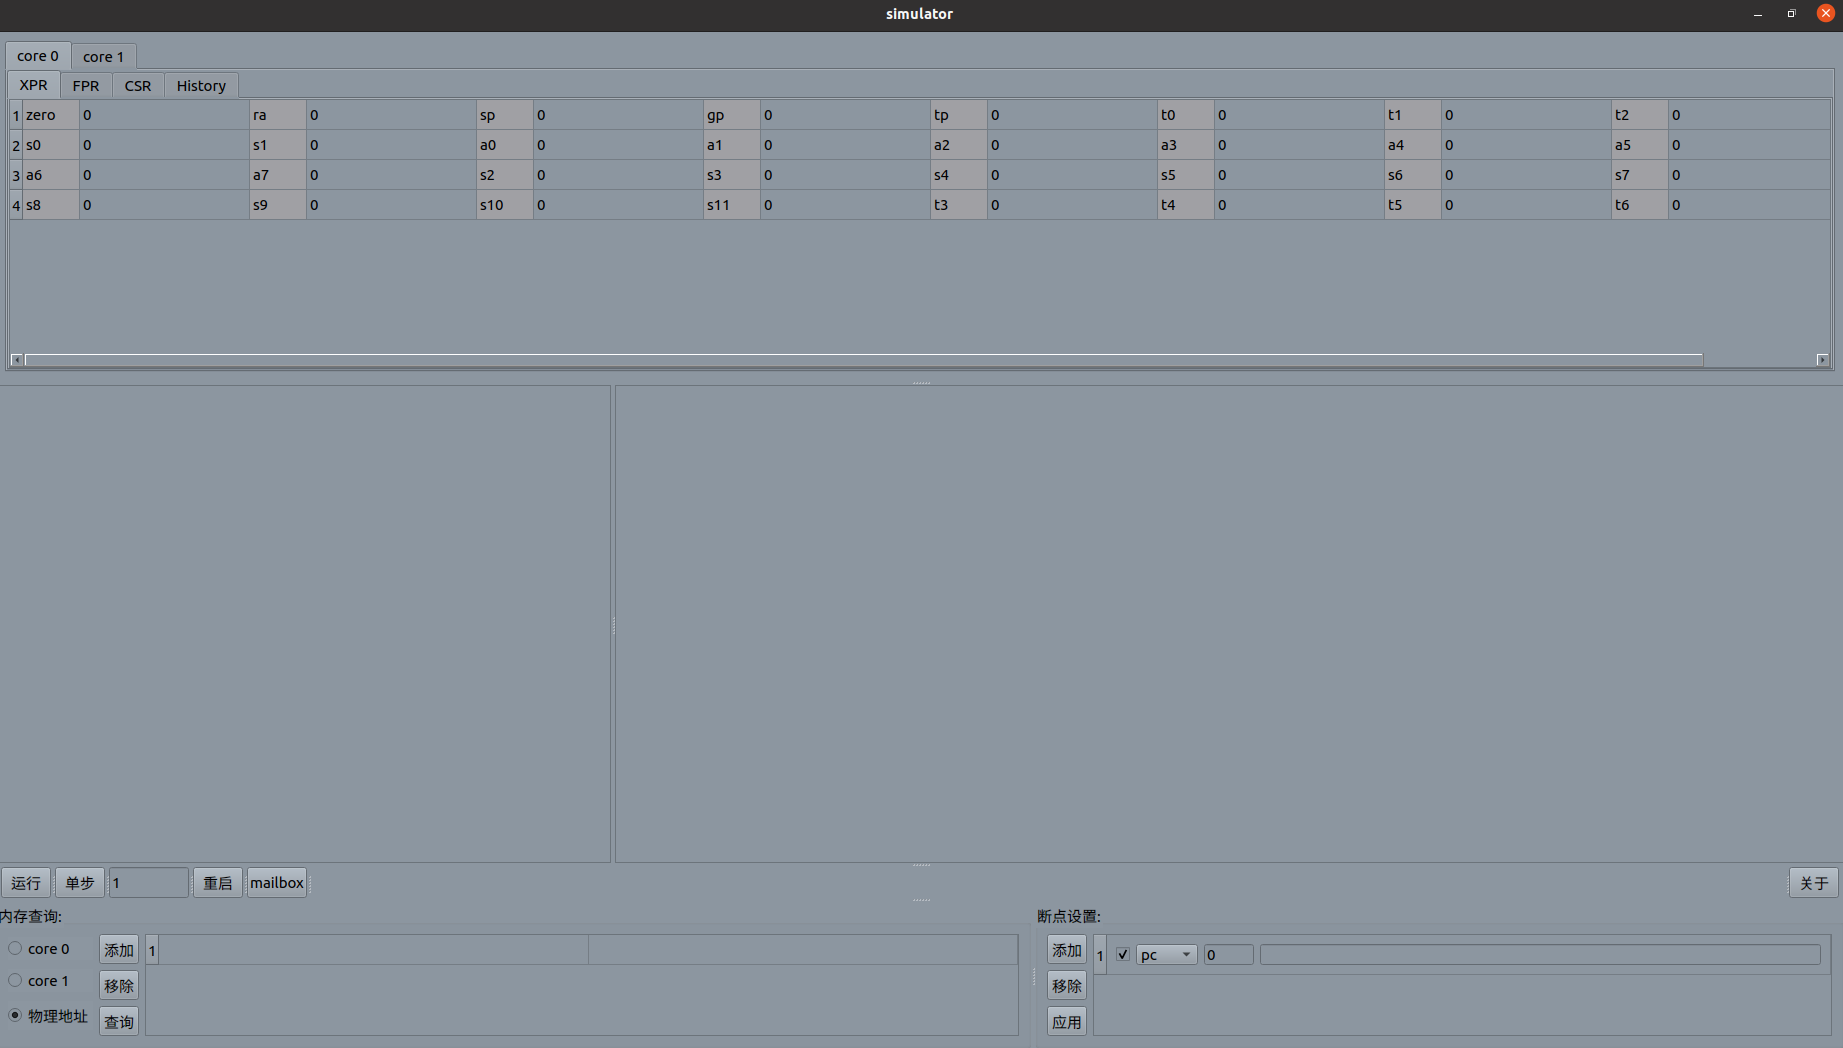
\includegraphics[width=1.0\textwidth]{zhenti.png}
    \caption{模拟器前端整体界面}
    \label{fig:zhenti}
\end{figure}


断点设置窗口如图所示,可以添加任意多个断点,断点匹配类型分为如下几种:PC,寄存器,内存,中断类型。当模拟器包含多核时需要指定相应的核心ID号。当模拟器处于调试模式时,中断指令流程,此时可以进行断点设置,内存查询等操作,点击运行按键,模拟器恢复至正常运行模式,在每一次指令执行周期完成后模拟器将对当前断点信息进行检查,一旦匹配上任意断点,将发送window\_cmd\_sim\_output信号用于告知触发断点信息,并接着发送window\_cmd\_pause\_sim信号,中断指令流程,模拟器进入调试模式。每发送一次单步执行信号,模拟器都需要将寄存器更新信号发送给UI前端,刷新寄存器窗口。


模拟器单步执行的流程如图~\ref{fig:step}所示。
\begin{figure}[H]
    \centering
    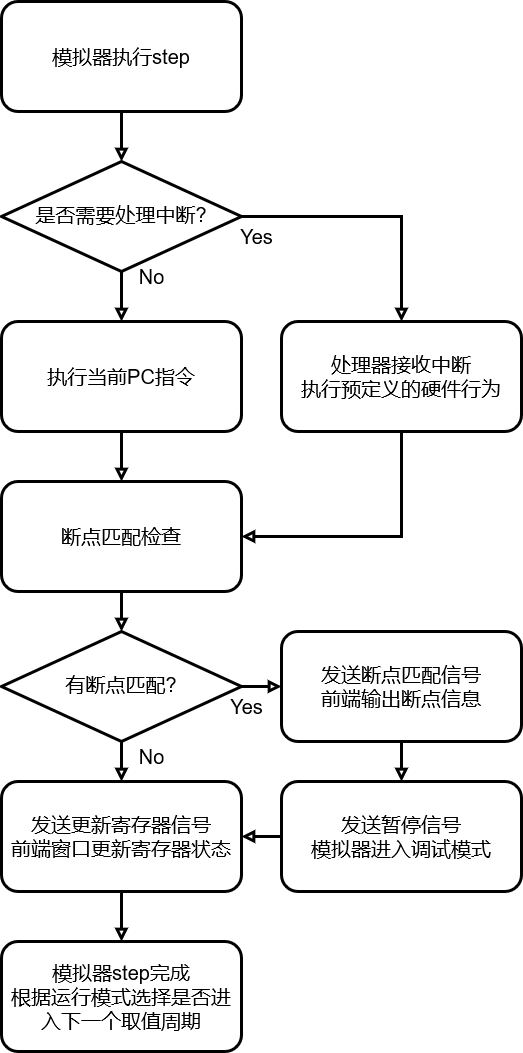
\includegraphics[width=0.5\textwidth]{step-logic.png}
    \caption{调试模式下单步执行流程}
    \label{fig:step}
\end{figure}


\section{本章小结}
本章主要在概要设计的基础上对RISC-V指令集模拟器四个功能模块的详细设计和实现细节进行了阐述,并根据实际工程项目中使用的设备和具体型号IP文档,进行了部分外设的功能模拟,验证了模拟器的可用性,最后完成了前后端所有功能模块的代码实现,并给出了相应的演示效果图.


